\documentclass[11pt,oneside]{article}
\usepackage[T1]{fontenc}
\usepackage[utf8]{inputenc}
%\DeclareUnicodeCharacter{00A0}{ }
\usepackage[adobe-utopia]{mathdesign}

\usepackage{amsmath}
\usepackage[francais]{babel}
\usepackage[dvips]{graphicx}
%\usepackage{here}
\usepackage{framed}
\usepackage[normalem]{ulem}
\usepackage{fancyhdr}
\usepackage{titlesec}
\usepackage{vmargin}

\usepackage{amsmath}
\usepackage{ifthen}
\usepackage{multirow}
\usepackage{multicol} % Portions de texte en colonnes

%\usepackage{xltxtra} % Logo XeLaTeX
%\usepackage{pst-solides3d}
\usepackage{color}
%\usepackage{colortbl}
\usepackage{titletoc} % Pour la mise en forme de la table des matières

%\usepackage[crop=off]{auto-pst-pdf}
%\usepackage{bclogo}


%\usepackage{longtable}
%\usepackage{flafter}%floatants après la référence
%\usepackage{pst-solides3d}
%\usepackage{pstricks}
%\usepackage{minitoc}
%\setcounter{minitocdepth}{4}
%\usepackage{draftcopy}% "Brouillon"
%\usepackage{floatflt}
%\usepackage{psfrag}
%\usepackage{listings} % Permet d'insérer du code de programmation
%\usepackage{lmodern}
%\usepackage[adobe-utopia,uppercase=upright,greeklowercase=upright]{mathdesign}
%\usepackage{minionpro}
%\usepackage{pifont}
%\usepackage{amssymb}
%\usepackage[francais]{varioref}

\setmarginsrb{1.5cm}{1cm}{1cm}{1.5cm}{1cm}{1cm}{1cm}{1cm}

\definecolor{gris25}{gray}{0.75}
\definecolor{bleu}{RGB}{18,33,98}
\definecolor{bleuf}{RGB}{42,94,171}
\definecolor{bleuc}{RGB}{231,239,247}
\definecolor{rougef}{RGB}{185,18,27}
\definecolor{rougec}{RGB}{255,230,231}
\definecolor{vertf}{RGB}{103,126,82}
\definecolor{vertc}{RGB}{220,255,191}
\definecolor{violetf}{RGB}{112,48,160}
\definecolor{violetc}{RGB}{230,224,236}
\definecolor{jaunec}{RGB}{220,255,191}
\usepackage[raccourcis]{FAST}
\usepackage[%
    pdftitle={IS -- SysML -- Diagramme des exigences},
    pdfauthor={Xavier Pessoles},
    colorlinks=true,
    linkcolor=blue,
    citecolor=magenta]{hyperref}

\usepackage{pifont}


% \makeatletter \let\ps@plain\ps@empty \makeatother
%% DEBUT DU DOCUMENT
%% =================
\sloppy
\hyphenpenalty 10000

\newcommand{\Pointilles}[1][3]{%
\multido{}{#1}{\makebox[\linewidth]{\dotfill}\\[\parskip]
}}


\colorlet{shadecolor}{orange!15}

\newtheorem{theorem}{Theorem}


\begin{document}


\newboolean{prof}
\setboolean{prof}{true}
%------------- En tetes et Pieds de Pages ------------
\pagestyle{fancy}
\renewcommand{\headrulewidth}{0pt}

\fancyhead{}
\fancyhead[L]{%
\noindent\noindent\begin{minipage}[c]{2.6cm}
%Lycée Rouvière PTSI

\includegraphics[width=2cm]{png/logo_ptsi.png}%
\end{minipage}
}


\fancyhead[C]{\rule{12cm}{.5pt}}

\fancyhead[R]{%
\noindent\begin{minipage}[c]{3cm}
\begin{flushright}
\footnotesize{\textit{\textsf{Sciences Industrielles\\ de l'Ingénieur}}}%
\end{flushright}
\end{minipage}
}

\renewcommand{\footrulewidth}{0.2pt}

\fancyfoot[C]{\footnotesize{\bfseries \thepage}}
\fancyfoot[L]{\footnotesize{2013 -- 2014} \\ X. \textsc{Pessoles}}
\ifthenelse{\boolean{prof}}{%
\fancyfoot[R]{\footnotesize{CI 1 : IS -- Cours \\
Ch 3 SysML -- Exigences -- P}}
}{%
\fancyfoot[R]{\footnotesize{Cours -- CI 6 : PPM}}
}



\begin{center}
 \huge\textsc{CI 1 -- IS}

 \large\textsc{Étude des systèmes pluritechniques et multiphysiques -- Initiation à l'Ingénierie Système}
\end{center}

\begin{center}
 \LARGE\textsc{Chapitre 3 -- SysML -- Diagramme des exigences}
\end{center}

%\begin{flushright}
%\textit{D'après documents de Jean-Pierre Pupier}
%\end{flushright}

\vspace{.5cm}





%\begin{minipage}[c]{.23\linewidth}
%\begin{center}
%\includegraphics[height=2.5cm]{png/tour_bois}
%
%\textit{Tour à bois \cite{tab}}
%\end{center}
%\end{minipage} \hfill
%\begin{minipage}[c]{.23\linewidth}
%\begin{center}
%\includegraphics[height=2.5cm]{png/cazeneuve}
%
%\textit{Tour conventionnel \cite{cazeneuve}}
%\end{center}
%\end{minipage} \hfill
%\begin{minipage}[c]{.23\linewidth}
%\begin{center}
%\includegraphics[height=2.5cm]{png/tour_mazak}
%
%\textit{Tour à commande numérique \cite{mazak}}
%\end{center}
%\end{minipage}\hfill
%\begin{minipage}[c]{.23\linewidth}
%\begin{center}
%\includegraphics[height=2.5cm]{png/plaquettes}
%
%\textit{Plaquettes de tournage \cite{plaquettes}}
%\end{center}
%\end{minipage}

\vspace{.5cm}

\begin{center}
%\includegraphics[height=7cm]{png/cycleV}
\end{center}

%\begin{center}
%\includegraphics[width=.9\textwidth]{png/cyclev.png}

%\textit{Cycle de conception d'un produit}
%\end{center}

%\begin{prob}
%\textsc{Problématique :}
%\begin{itemize}
%\item %Quelles sont les conditions fonctionnelles permettant le fonctionnement du système ?
%\item %Quelle est la chaîne de côte unidirectionnelle correspondant à une condition donnée ?
%\end{itemize}
%\end{prob}



\begin{savoir}
\textsc{Savoirs}
\begin{itemize}
%\item A-C1.1 : Besoin, système, services attendus du système, cahier des charges fonctionnel, spécifications fonctionnelles, analyse du cycle de vie, acteurs, interactions, solution technique.	
\item A-C1-S1 : Décomposer une exigence en plusieurs exigences unitaires
\item A-C1-S2 : Identifier des exigences de niveaux différents
\end{itemize}
\end{savoir}
 
Le diagramme des exigences (\textit{requirement diagram}) permet de lister toutes les exigences auxquelles le système doit répondre.

\begin{center}
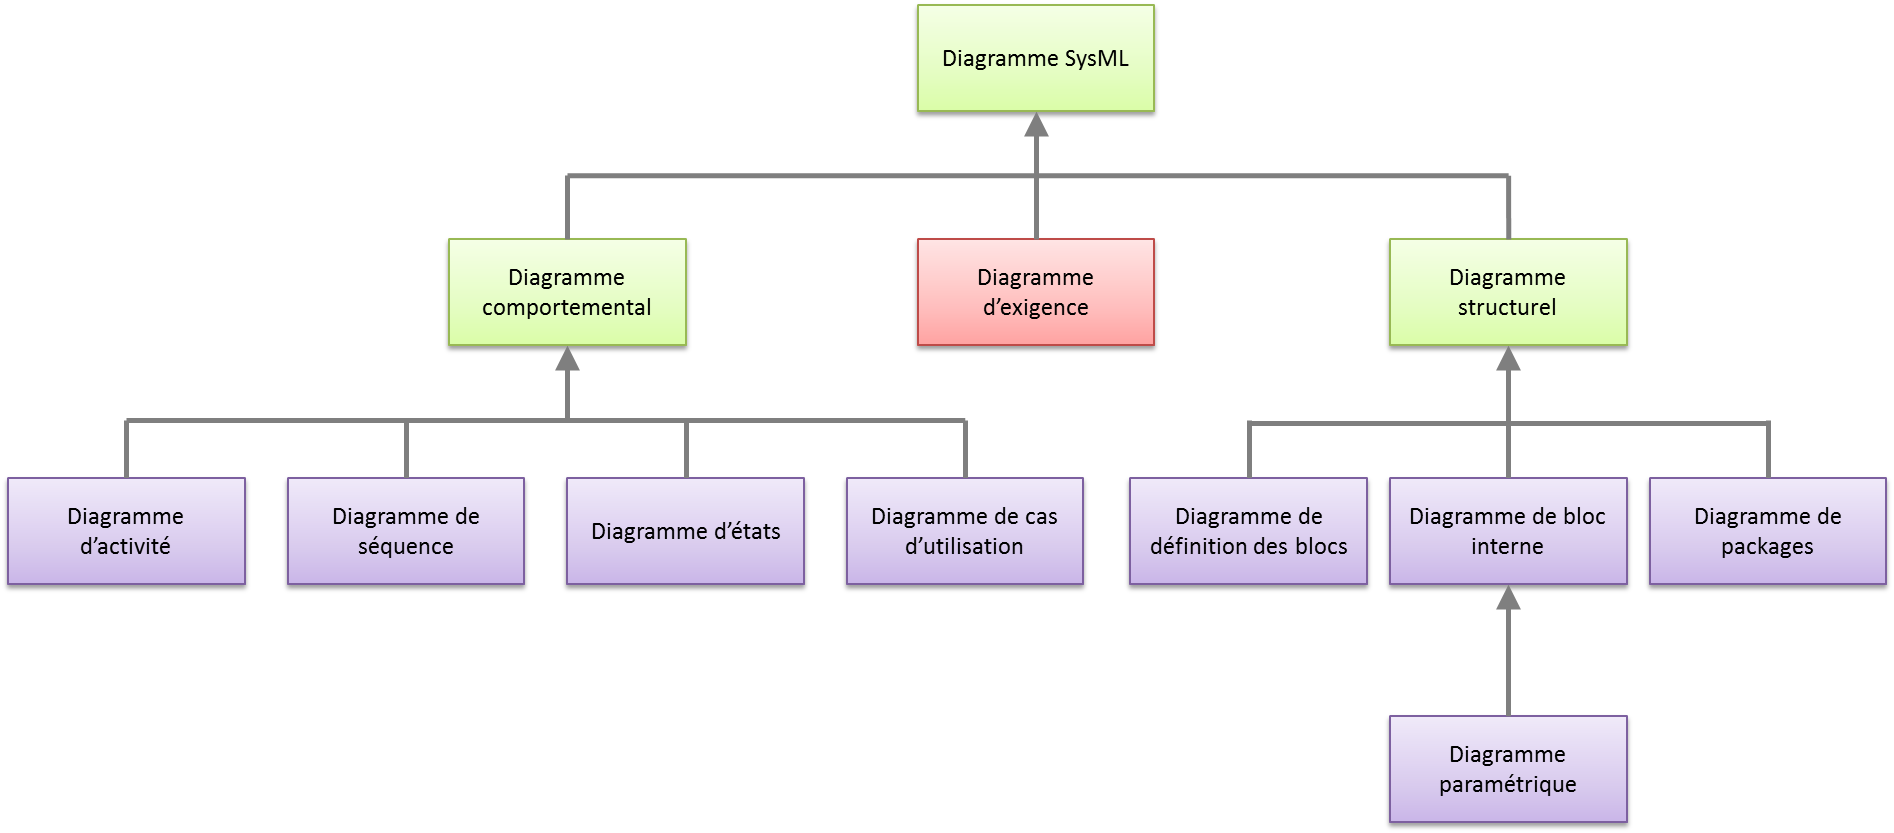
\includegraphics[width=0.9\textwidth]{png/diagrammes}
\end{center}


\setlength{\parskip}{0ex plus 0.2ex minus 0ex}
 \renewcommand{\contentsname}{}
 \renewcommand{\baselinestretch}{1}

\tableofcontents

 \renewcommand{\baselinestretch}{1.2}
\setlength{\parskip}{2ex plus 0.5ex minus 0.2ex}

% \vspace{1cm}
\textit{Ce document évolue. Merci de signaler toutes erreurs ou coquilles.}

\section{Présentation}

\begin{defi}
\textbf{Exigences} --  \textit{Requirement} -- \textit{req} \cite{roques}

Une exigence permet de spécifier une capacité ou une contrainte qui doit être satisfaite par un système.
Elle peut spécifier une fonction que le système devra réaliser ou une condition de performance,
de fiabilité, de sécurité, etc.

Les exigences servent à établir un contrat entre le client et les réalisateurs du futur système.


Une exigence est représentée par un cadre sur lequel sont précisés :
\begin{itemize}
\item \textit{requirement};
\item le nom de l'exigence;
\item un identifiant unique;
\item une description textuelle de l'exigence si son nom n'est pas assez explicite.
\end{itemize}
\end{defi}

\begin{exemple}
\textit{Exigence sur l'accélération d'un véhicule}

\begin{center}
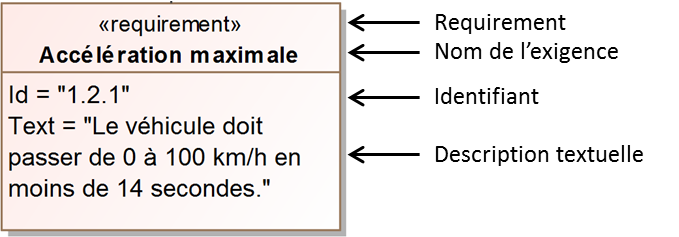
\includegraphics[width=.4\textwidth]{png/exigence}
\end{center}
\end{exemple}



\begin{exemple}
\begin{center}
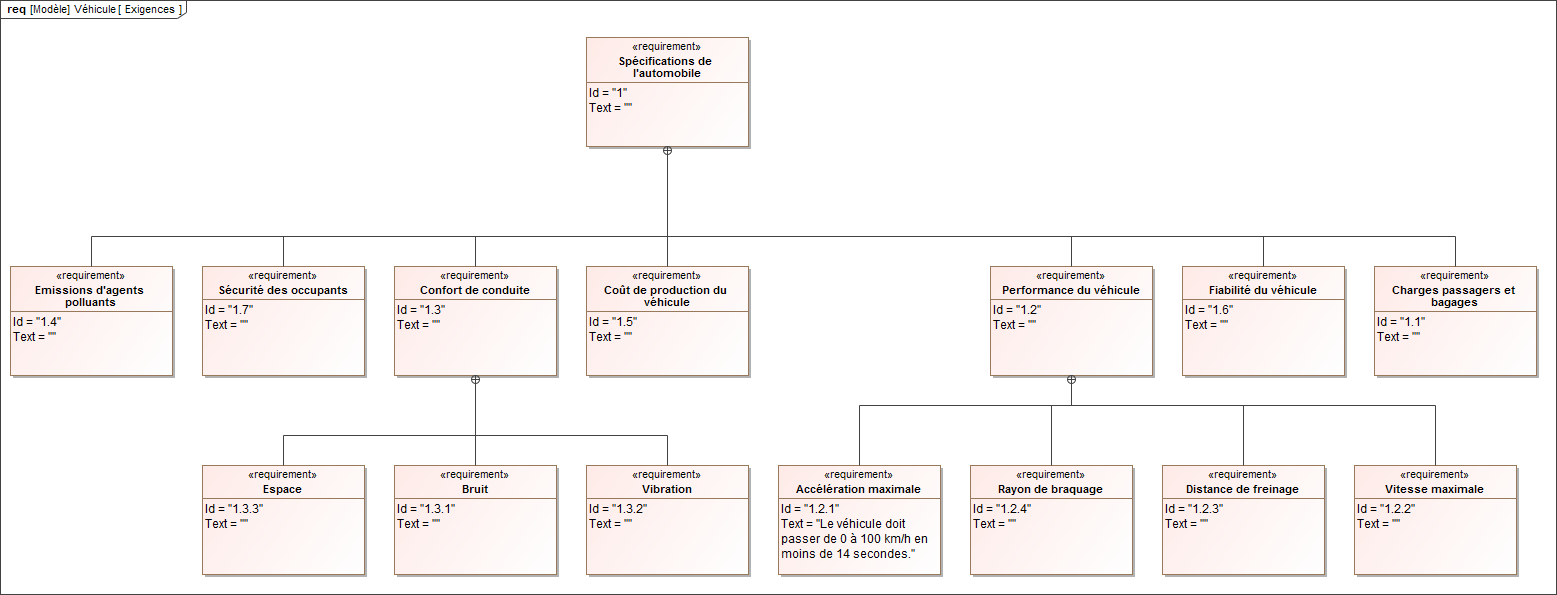
\includegraphics[width=\textwidth]{png/DiagrammeExigences}
\end{center}
\end{exemple}


\begin{rem}
Dans le but de réaliser une structuration des exigences, il est possible de définir des "macro exigences" telles que : 
\begin{itemize}
\item les exigences fonctionnelles;
\item les exigences légales;
\item les exigences environnementales;
\item les exigences techniques;
\item les exigences pratiques;
\item les exigences énergétiques;
\item les exigences marketing.
\end{itemize}
\end{rem}


\subsection{Relation entre les exigences}

\begin{defi}
\textbf{Relation de contenance}

Décomposition d'une "macro" exigence en exigences plus élémentaires

\begin{minipage}[c]{.6\linewidth}
\end{minipage} \hfill
\begin{minipage}[c]{.3\linewidth}
\begin{center}
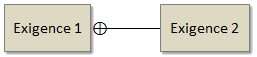
\includegraphics[width=.9\textwidth]{png/cont}
\end{center}
\end{minipage}

\end{defi}
Le rond indique l'exigence d'origine.



\begin{defi}
\textbf{Raffinement -- \textit{refine}}

Relation permettant de rajouter des précisions (données quantitatives par exemple). 

\begin{minipage}[c]{.6\linewidth}
\end{minipage} \hfill
\begin{minipage}[c]{.3\linewidth}
\begin{center}
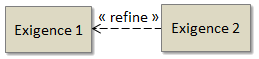
\includegraphics[width=.9\textwidth]{png/ref}
\end{center}
\end{minipage}
\end{defi}

L'exigence fille précise l'exigence mère. 

\begin{defi}
\textbf{Dérivation -- \textit{deriveReqt}}

Permet de relier des exigences de niveaux différents. 

\begin{minipage}[c]{.6\linewidth}
\end{minipage} \hfill
\begin{minipage}[c]{.3\linewidth}
\begin{center}
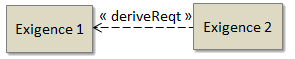
\includegraphics[width=.9\textwidth]{png/derivreq}
\end{center}
\end{minipage}

\end{defi}

L'exigence fille est déduite de l'exigence mère. Cette exigence n'est pas émise par le client en tant que tel, mais peut être une exigence induite par plusieurs exigences. 


\begin{minipage}[c]{.5\linewidth}
Imagerie médicale -- mécanisme de positionnement
\end{minipage} \hfill
\begin{minipage}[c]{.3\linewidth}
\begin{center}
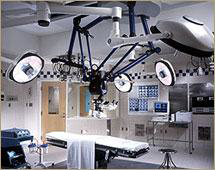
\includegraphics[width=.9\textwidth]{png/imagerie}
\end{center}
\end{minipage}


\begin{center}
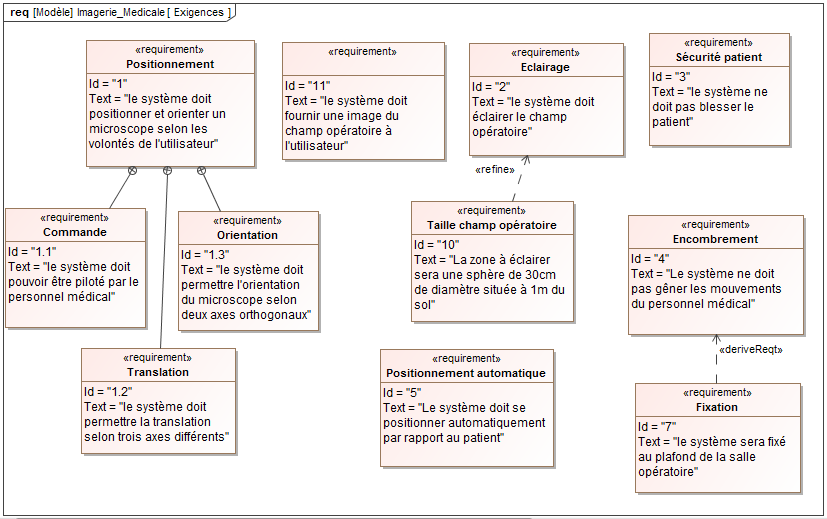
\includegraphics[width=.9\textwidth]{png/imagerie_req}
\end{center}

\section{Pour aller plus loin}
\subsection{Notion de tracabilité}
Afin de justifier certaines solutions technologiques qui ont été adoptées, ou pour permettre le suivi et les conséquences des évolutions de certains constituants du système ou des modifications d’architecture, on peut faire apparaître des liens entre les exigences et d’autres objets, tels :
\begin{itemize}
\item « refine » : l’objet permet de préciser l’exigence, par un cas d’utilisation, un diagramme de séquence ou un diagramme d’états (sui seront vus en fin d’année);
\item « satisfy » : l’objet permet de préciser quel est le composant ou l’algorithme qui permet de satisfaire l’exigence.
Ces liens peuvent être définis dans un autre diagramme d’exigence par exemple.
\end{itemize}

\begin{center}
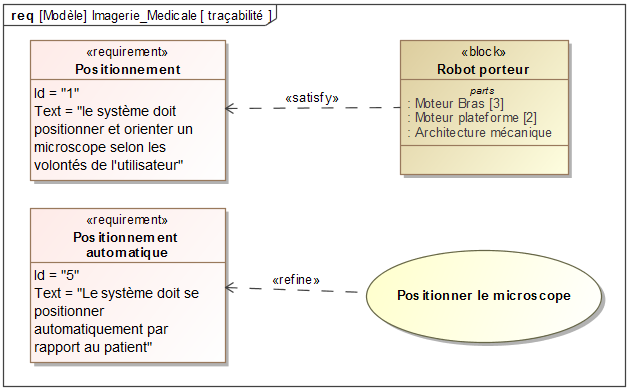
\includegraphics[width=.8\textwidth]{png/tracabilite}
\end{center}

\begin{thebibliography}{2}
\bibitem{roques}{Pascal Roques, SysML par l'exemple -- Un langage de modélisation pour systèmes complexes. Éditions Eyrolles, 2009.}
\bibitem{debout}{Pierre Debout, SII -- Analyse Externe des systèmes.}
\bibitem{martin}{Beaudoin Martin, Formation SysML.}
\bibitem{martin2}{Beaudoin Martin, Construction	du	modèle	SysML	de	la	balance	
HALO	de	chez	Terraillon.}
\bibitem{martin3}{Beaudoin Martin, Diagrammes SysML -- L'essentiel en STI2D.}
\bibitem{sanford}{Sanford Friedenthal, Alan Moore, Rick Steiner, A Practical Guide to SysML-- The Systems Modeling Language. Elsevier, 2008.}
\bibitem{cmartin}{Carole Martin, Etude des Systèmes -- Communication technique}
\end{thebibliography}

\end{document}
